\documentclass[a4paper,12pt]{article}
\usepackage{graphicx}
\graphicspath{ {images/} }

% Language and font encodings
\usepackage[utf8]{inputenc}
\usepackage[american]{babel}

% Specify bibliography package
\usepackage{csquotes}% Recommended
\usepackage[style=apa]{biblatex}
\DeclareLanguageMapping{american}{american-apa}
\addbibresource{references.bib}

% Sets page size and margins
\usepackage[top=2cm,bottom=2cm,left=2cm,right=2cm,marginparwidth=1.75cm]{geometry}
\setlength{\parskip}{1em}

% package for formatting and highlighting source code
\usepackage{listings}
\usepackage{color}

% Useful packages
\usepackage{amsmath}
\usepackage{graphicx}
\usepackage{float}
\usepackage[colorlinks=true, allcolors=black]{hyperref}
\usepackage{graphicx}
\usepackage{setspace}

% packages for tikz diagrams
\usepackage{tikz}
\usetikzlibrary{shapes.geometric, arrows}

% styling for tikz diagrams
\tikzstyle{startstop} = [rectangle, rounded corners, minimum width=10cm, minimum height=1cm,text centered, text width=10cm, draw=black, fill=gray!10]
\tikzstyle{process} = [rectangle, minimum width=10cm, minimum height=1cm, text centered, text width=10cm, draw=black, fill=orange!30]
\tikzstyle{arrow} = [thick,->,>=stealth]

% List of abbreviations
\usepackage {acronym}

% Section Title Margins
\usepackage{titlesec}
\titlespacing*{\section}
{0pt}{3.0ex plus 1ex minus .2ex}{0.7ex}
\titlespacing*{\subsection}
{0pt}{1.4ex}{0pt}
\definecolor{dkgreen}{rgb}{0,0.6,0}
\definecolor{gray}{rgb}{0.5,0.5,0.5}
\definecolor{mauve}{rgb}{0.58,0,0.82}

\lstset{frame=tb,
  language=Python,
  aboveskip=3mm,
  belowskip=3mm,
  showstringspaces=false,
  columns=flexible,
  basicstyle={\small\ttfamily},
  numbers=none,
  numberstyle=\tiny\color{gray},
  keywordstyle=\color{blue},
  commentstyle=\color{dkgreen},
  stringstyle=\color{mauve},
  breaklines=true,
  breakatwhitespace=true,
  tabsize=3}

\title{Your Title Goes Here}
\author{Your Name Goes Here}

%************************** DOCUMENT_STARTS_HERE **************************
\begin{document}

\begin{titlepage}
	\begin{figure}
	\centering
	
\includegraphics[scale=0.32]{logohsg}
	\end{figure}
\centering
\centering
{\scshape\large School of Management, Economics, Law, Social Sciences and International Affairs \par}
\vspace{1.7cm}
{\huge\bfseries The effect of Twitter activity on \\ Bitcoin price\par}
\vspace{1.0cm}
{\Huge\itshape Documentation\par}
\vspace{1.0cm}     
{\Large Software Engineering for Economists \\ (7,610,1.00) \par}
\vspace{1.2cm}
{Alen Stepic - 11-475-258 \\ Dimitrios Koumnakes - 10-613-370 \\ Severin Kranz - 13-606-355 \\ Joël Sonderegger - 11-495-488 \\ Chi Xu - XX-XXX-XXX \par}
\vspace{1.2cm}
Fall Term 2017 \\
\vspace{1.2cm}
{Supervisor\\ Prof. Dr. Philipp Zahn\\ FGN HSG\\ Varnbüelstrasse 19\\ 9000 St. Gallen\\ Department of Economics\par}
\vspace{0.8cm}
{\centering\today\par}
\end{titlepage}

\clearpage

\tableofcontents

\clearpage
    
    \listoffigures\bigskip 
    \section*{List of Abbreviation} 
	\begin{acronym}[ASECRETTT] 
	\acro{API}{Application Programming Interface}
	\acro{ATOKEN}{Access Token}
	\acro{ASECRET}{Access Token Secret}
	\acro{BPI}{Bitcoin Price Index}
	\acro{BTC}{Bitcoin}
	\acro{CKEY}{Consumer Key}
	\acro{CSECRET}{Consumer Secret}
	\acro{JSON}{Java Script Object Notation}
	\acro{RPI}{Raspberry Pi}
	\acro{SSH}{Secure Shell}
	\acro{USD}{US Dollar}
	\end{acronym}
    \clearpage



\begin{spacing}{1.2}
\cleardoublepage\pagenumbering{arabic}
\section{Introduction}
In the academic environment accountability and reproducibility is important. However, the publishing process of papers and journals seem to be outdated as reproducability is not evaluated by many journals. \parencite[p.~888]{mccullough2003} New ways of data collection and data processing exist by using computational economics. The usage of algorithms can increase effectiveness and efficiency. Hence, much lager data sets can be proceeded. However this creates also new problems regarding to traceability and reproducibility. Often cited academic paper exist, where the initial computation is not reproducible \parencite[pp.~874--887]{mccullough2003}. Replicating data or existing results do not provide any new knowledge at all. Nevertheless, the ability to reproduce is key in science and non-reproducable work can not be characterized as science or used as a basis for policy making \parencite[p.~888]{mccullough2003}. This explains why reproduction is of great relevance.

\subsection{Goal of the paper}
The goal of this documentation is the provision of a description. This description should enable the reader to reproduce the results discussed in the separate paper. Thus, it contains an explanation how the input data have been gathered, stored, aggregated and analysed. In other words, the input data, the model core, the model parameters and the applied math program are explained.

\subsection{Methodology}
This documentation consists out of four chapters. The first chapter contains a short introduction and provides the reader with an overview about the topic. Furthermore it points out the relevance of documentation. The second chapter discusses the input data. This includes the process of gathering and storing twitter tweets as well as the gathering of the bitcoin price data. The third chapter discusses how the data is aggregated by pointing out the core model and its parameters. Finally the fifth chapter discusses how the analysis has been conducted.

\subsection{Scope}
The scope of the documentation is the provision of an overview about the different steps which have been conducted to obtain the results in the paper. It does not contain any discussions about the results of the separate paper. It is not a deep description of the code as the code itself as the code is documented separately. Nevertheless, important lines of code are discussed. 
\clearpage

\section{Setup}
\subsection{Requirements to run Python scripts}
Before you go any further, make sure that at least Python version 3.0.0 available from your command line. You can check this by running:
\begin{lstlisting}[language=bash]
    python --version
\end{lstlisting}
You should get some output like Python 3.7.13. If you do not have at least Python version 3.0.0, please install the latest 3.x version from python.org.
\newline
On top you need various packages. We created a the requirements file \verb|requirements.txt|, which contains all required packages to run Python scripts of the project. The list of packages to be installed using pip install like so:
\begin{lstlisting}[language=bash]
    pip install -r requirements.txt
\end{lstlisting}
Now you should be ready to run the Python scripts.

\subsection{Stata}
For the data analysis, we used the statistical software STATA (version 14.2). When seeking for statistical analysis, regression analysis or data management, STATA is a capable tool. To reproduce our results, you need to have the STATA software installed in your local computer and after starting the program you can follow the guidelines in chapter 4 (data analysis). 

\section{Data Collection}
This section contains a detailed description of how the data for the sequential analysis is gathered and stored. This includes two  subsections the (1) tweets data and the (2) bitcoin price data.
\subsection{Tweets Data}
Whit the python script real-time twitter data are streamed and stored. This happens with help of a raspberry pi.
\subsubsection{Python Script}
Twitter offers different Application Programming Interfaces (API) for collecting data. However, the time frame for gathering data on a freely base with full access is limited to 7 days \parencite{twitterinc2017a}. On the other hand, python offers different twitter libraries. Such as the open-source package tweepy. This package has been used for streaming the twitter data as it simplify the script.

\paragraph{Installing Tweepy}\mbox{}\\{}
Tweepy is installed very simply by running following commands in the command prompt. 
\begin{lstlisting}[language=bash]
pip install tweepy
\end{lstlisting}

If the previous downloaded python installation package does not contain the tweepy library, the tweepy package has to be downloaded. The package can be downloaded for free from the following link:
\begin{lstlisting}[language=bash]
https://pypi.python.org/pypi/tweepy
\end{lstlisting}

\paragraph{Twitter Authentication}\mbox{}\\{}
To access the twitter data, twitter requests an identification of the user. The identification is assured by different keys and access tokens. Those are the (1) consumer key (CKEY), (2) consumer secret (CSECRET), (3) access token (ATOKEN) and (4) access token secret (ASECRET). \parencite{twitterinc2017b}

To obtain the mentioned keys and tokens a twitter account is needed. Once, a twitter account exist a application has to be created. This has to be conducted by login with the twitter account credentials under the following link: 
\begin{lstlisting}[language=bash]
%https://apps.twitter.com/
\end{lstlisting}

After the creation of a application, the keys and tokens can be extracted. Figure \ref{figkeysandtokens} illustrates how to retrieve the keys and tokens.
\begin{figure}[H]
\centering
	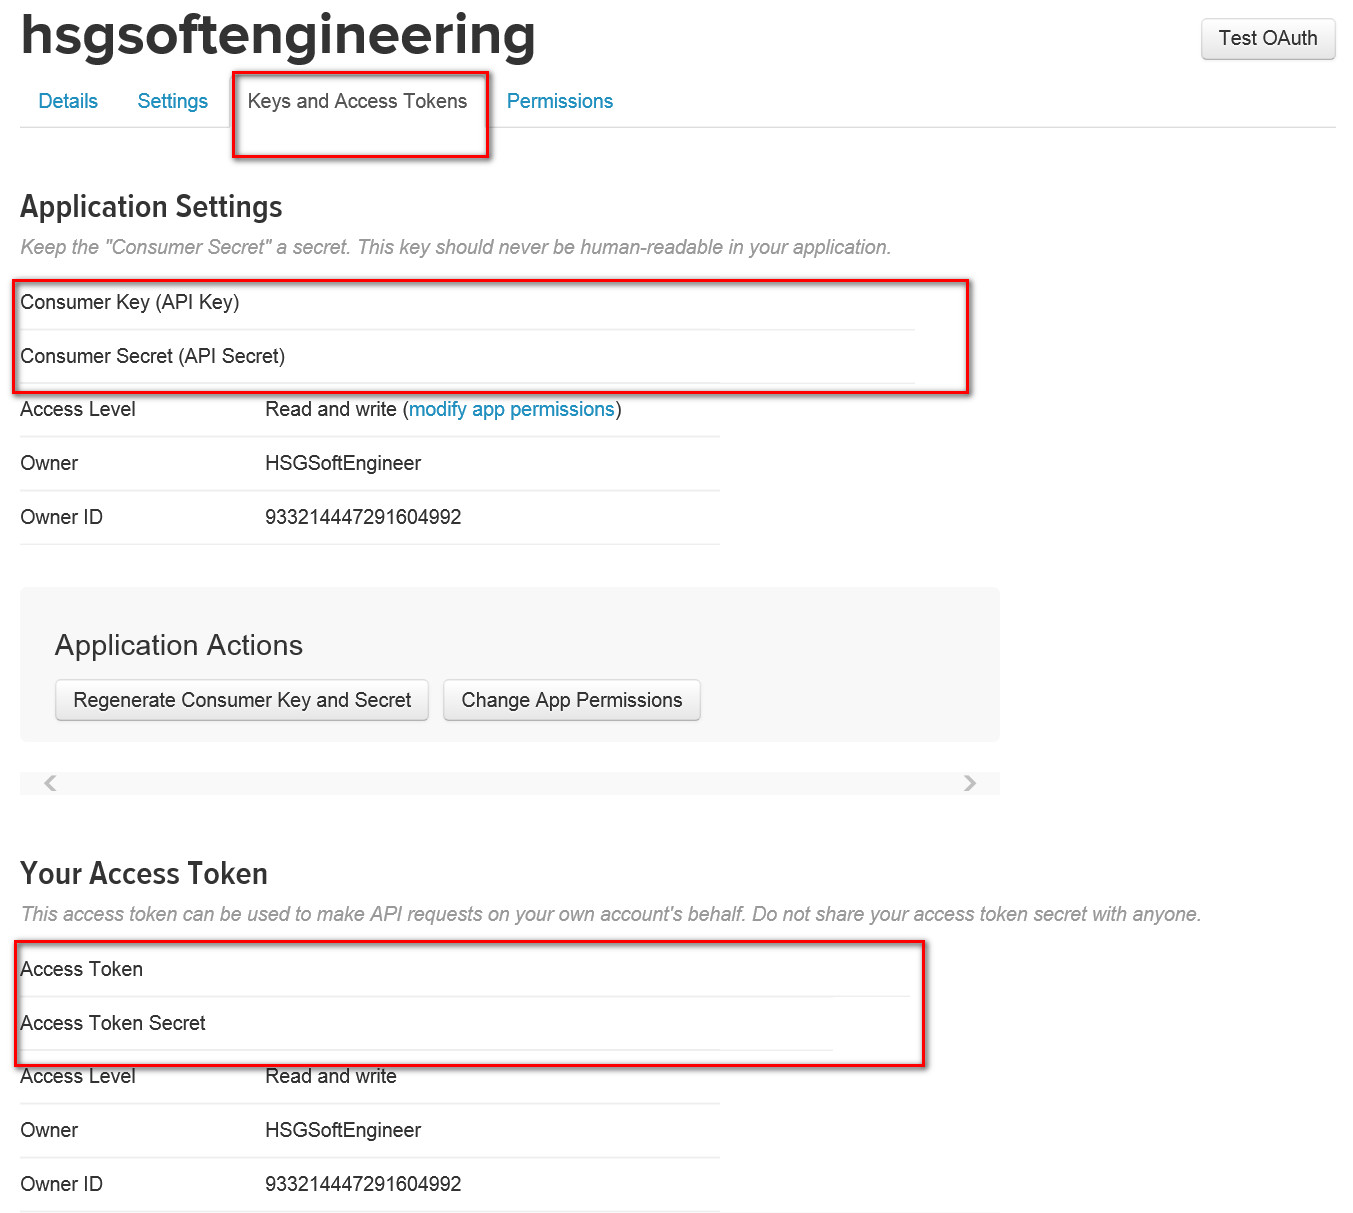
\includegraphics[scale=0.6]{twitteraccess}
\caption{Twitter Keys and Access Tokens, based on \textcite{twitterinc2017c}.}
	\label{figkeysandtokens}
\end{figure}

\paragraph{Twitter Streaming API}\mbox{}\\{}
By running the python script \verb|collectTwitterData.py| real-time twitter data is pushed in a Java Script Object Notation (JSON) format. Tweets are just pushed in case a tweet contains the defined key word \verb|bitcoin|.
\begin{lstlisting}[language=bash]
$ python collectTwitterData.py
\end{lstlisting}

From the JSON format the following parameters are decoded:
\begin{itemize}
    \item created at: Timestamp of the created tweet
    \item text: Text of the tweet
\end{itemize}
The timestamps are in UTC time.

After a successfully decoding the parameters the data is appended to the \verb|twitterData.csv| file in a new row and saved in the folder \verb|/data|.

An excerpt of an example response looks like the following:
\begin{lstlisting}
[
    {
        "created_at": Tue Dec 19 20:40:48 +0000 2017, 
        "text": "RT @WhiteBitcoin: New Bitcoin White. Effective, Flexible, Reliable", 
    }, 
    {
        "created_at": Tue Dec 19 20:40:49 +0000 2017 ,
        "text": "As #bitcoin prices surge, #xrp remains affordable and FAST!",
    }, 
    {
        "created_at": Tue Dec 19 20:40:49 +0000 2017, 
        "text": "Singapore issues bitcoin warning after price rise - #BTC #Bitcoin #Crypto", 
    }
]
\end{lstlisting}

Furthermore to ensure a high quality data set an exception has been integrated into the \verb|collectTwitterData.py| script. If an error occurs an email will be sent with the error message. Furthermore the logfile will be  appended to \verb|/data/tweet_collection_error_log.csv|.

\subsubsection{Hardware Setup}
As explained in the previous section the twitter API was used to filter tweets in real time based on the buzzword \"bitcoin\". The Python program was running for seven days without interruption on a Raspberry Pi 2 (RPI) which was accessed with a Secure Shell (SSH) connection. This approach allowed us to ensure a continuous data stream while being able to access the program output regardless of time and location. Furthermore, due to a low energy consumption of the RPI the method is also the most cost efficient one compared to a personal computer or NAS Server. The following section describes the different steps that have been taken in order to setup the RPI 2, SSH, Git and Python3.\newline 

\begin{enumerate}
\item Setup of the Raspberry Pi
\begin{enumerate}
\item Burn image 2017-11-29-raspbian-stretch.zip to micro SD card available from
\begin{lstlisting}[language=bash]
https://www.raspberrypi.org/downloads/raspbian/
\end{lstlisting}
\item Boot image from micro SD card 
\item Open SSH session using PuTTY SSH client for Windows available from
\begin{lstlisting}[language=bash] 
https://www.chiark.greenend.org.uk/~sgtatham/putty/latest.html
\end{lstlisting}
\item Login to server with credentials 
\end{enumerate}

\item Update system to the newest software
\begin{enumerate}
\item Update list of applications with the command
\begin{lstlisting}[language=bash]
sudo apt-get update
\end{lstlisting}
\item Update applications with the command
\begin{lstlisting}[language=bash]
sudo apt-get upgrade
\end{lstlisting}
\end{enumerate}

\item Setup Git
\begin{enumerate}
\item Install Git using the command
\begin{lstlisting}[language=bash]
 sudo apt-get install git
\end{lstlisting}
\item Clone Git repository from
\begin{lstlisting}[language=bash] 
https://github.com/joelsonderegger/twitterbitcoin.git
\end{lstlisting}
\end{enumerate}

\item Setup Python3
\begin{enumerate}
\item Install Python3 using the command: sudo apt-get install Python3 \newline
\item Install the tweepy module for python using the command
\begin{lstlisting}[language=bash]
pip install tweepy
\end{lstlisting}
\end{enumerate}

\item Collect Twitter Data
\begin{enumerate}
\item Open a new screen using the command
\begin{lstlisting}[language=bash] 
screen -S 'name' 
\end{lstlisting}
\item Start Python program using the command
\begin{lstlisting}[language=bash]
python3 collectTwitterData.py
\end{lstlisting}
\item Detach the screen to keep the program running after secure shell connection has been terminated using the commands
\begin{lstlisting}[language=bash]
Ctrl+A
Ctrl+D
\end{lstlisting}
\item Re-attach the screen to check whether the script is still running using the command
\begin{lstlisting}[language=bash]
screen -r 'name'
\end{lstlisting}
\end{enumerate}

\item Download the collected data
\begin{enumerate}
\item Install FileZilla available from
\begin{lstlisting}[language=bash] 
https://filezilla-project.org/
\end{lstlisting}
\item Connect to rpi and navigate to data location \newline
\item Download data manually \newline \newline \end{enumerate}
\end{enumerate}
In summary, this approach worked well and ran smoothly. A clean setup is recommended to ensure a continuous data stream over a longer period.


\subsection{Bitcoin Price Data}
We wrote a Python script which collects Bitcoin price data as there was no preexisting data set that satisfied our needs. The Bitcoin price is best expressed by the Bitcoin Price Index. The Bitcoin price index (BPI) is an index of the exchange rate between the Bitcoin (BTC) and the US dollar (USD) (\cite{kristoufek2015main}). The objective of the script was to gather hourly Bitcoin Price Index data for at least the time period in which we gather the tweets data. We found the an API by bitcoinaverage.com which sufficed our needs. An API description follows later.

\subsubsection{Execution}
By executing the python script \verb|collectCryptocurrencyData.py| hourly data for the Bitcoin Price Index is retrieved.
\begin{lstlisting}[language=bash]
    $ python collectCryptocurrencyData.py
\end{lstlisting}

\subsubsection{Output}
After successfully running the python script \verb|CollectCryptocurrencyData.py| the file \verb|bpi.csv| is generated in the folder \verb|/data|. It is important to note that every execution of the script overwrites any existing \verb|bpi.csv| file.

The file \verb|bpi.csv| contains historical Bitcoin Price Index data for one month on an hourly basis. Each data point consists of the following parameters:
\begin{itemize}
    \item time: Timestamp on an hourly basis in UTC time
    \item average: Average price (in USD)
    \item high: Highest price (in USD)
    \item low: Lowest price (in USD)
    \item open: Opening price (in USD)
\end{itemize}

\subsubsection{API: Bitcoinaverage.com}
Bitcoinaverage.com offers a free API that provides real-time and historical price data for a range of crypto-currencies including Bitcoin. The following requests delivers data for an per hour monthly sliding window.
\paragraph{Request}\mbox{}\\
The request to get the data for an per hour monthly sliding window looks as follows. This request require authentication that requires registration and the generation of an API key. The registration and generation of an API key is freely available on bitcoinaverage.com. The collectCryptocurrencyData.py already contains the necessary keys. This means that you need no register or generate keys to execute the script collectCryptocurrencyData.py.  
\begin{lstlisting}[language=bash]
https://apiv2.bitcoinaverage.com/indices/global/history/BTCUSD?period=monthly&?format=json
\end{lstlisting}
\paragraph{Response}
An excerpt of an example response looks like the following:
\begin{lstlisting}
[
    {
        "high": 8271.04, 
        "average": 8247.83, 
        "open": 8242.39,
        "low": 8217.72, 
        "time": "2017-11-22 15:00:00"
    }, 
    {
        "high": 8246.82,
        "average": 8203.19,
        "open": 8203.81,
        "low": 8157.25,
        "time": "2017-11-22 14:00:00"
    }, 
    {
        "high": 8267.27, 
        "average": 8238.62, 
        "open": 8248.77, 
        "low": 8198.54, 
        "time": "2017-11-22 13:00:00"
    }
]
\end{lstlisting}


\section{Data Aggregation and Data Wrangling}
After the tweets and BPI data set is generated needs to be aggregated before it can be analyzed. In addition, some data wrangling is necessary to bring the data in a format which than can be analyzed. The script \verb|aggregateTwitterBpi.py| does all this.

\subsection{Process}
The process of the script \verb|aggregateTwitterBpi.py| works as follows:
\begin{figure}[H]
    \centering
    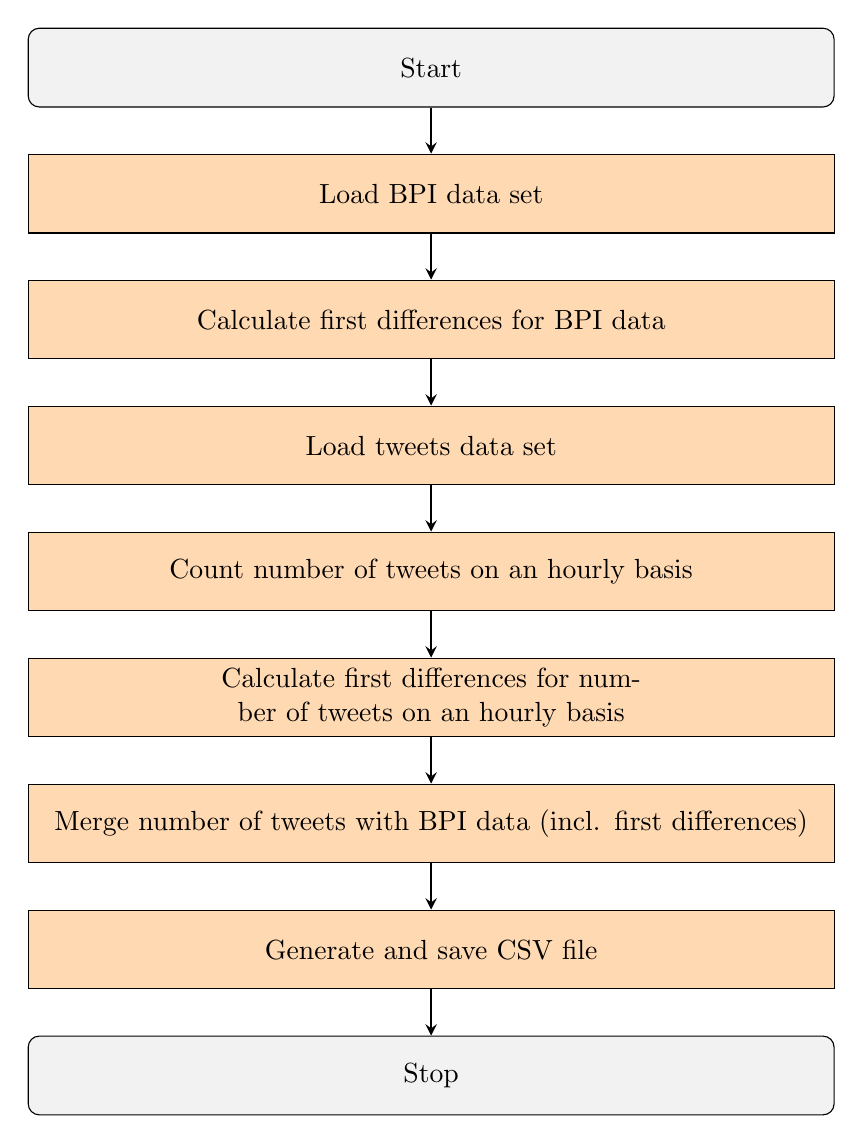
\begin{tikzpicture}[node distance=1.6cm]
        \node (start) [startstop] {Start};
        \node (pro1) [process, below of=start] {Load BPI data set};
        \node (pro2) [process, below of=pro1] {Calculate first differences for BPI data};
        \node (pro3) [process, below of=pro2] {Load tweets data set};
        \node (pro4) [process, below of=pro3] {Count number of tweets on an hourly basis};
        \node (pro5) [process, below of=pro4] {Calculate first differences for number of tweets on an hourly basis};
        \node (pro6) [process, below of=pro5] {Merge number of tweets with BPI data (incl. first differences)};
        \node (pro7) [process, below of=pro6] {Generate and save CSV file};
        \node (stop) [startstop, below of=pro7] {Stop};
        
        \draw [arrow] (start) -- (pro1);
        \draw [arrow] (pro1) -- (pro2);
        \draw [arrow] (pro2) -- (pro3);
        \draw [arrow] (pro3) -- (pro4);
        \draw [arrow] (pro4) -- (pro5);
        \draw [arrow] (pro5) -- (pro6);
        \draw [arrow] (pro6) -- (pro7);
        \draw [arrow] (pro7) -- (stop);
    \end{tikzpicture}
    \caption{Data aggregation and data wrangling process} \label{fig:dataaggregation}
\end{figure}

Here a short description of what happens at the various steps: 
\linebreak\linebreak
\textbf{Load BPI data set} The script takes the BPI data set that is located at \verb|data/bpi.csv|.
\linebreak\linebreak
\textbf{Calculate first differences for BPI data} The first differences of the BPI closing prices and the natural logarithm of the first differences of the BPI closing prices are calculated. The reason for calculating these values is given in the data analysis section.
\linebreak\linebreak
\textbf{Load tweets data set} The script takes the tweets data set that is located at \verb|data/twitterData.csv|.
\linebreak\linebreak
\textbf{Count number of tweets on an hourly basis} First, groups the tweets by hour. Second, counts the number of tweets for every hour.
\linebreak\linebreak
\textbf{Calculate first differences for number of tweets on an hourly basis} The first differences of the number of tweets and the natural logarithm of the first differences of the number of tweets are calculated. Again, the reason for calculating these values is given in the data analysis section.
\linebreak\linebreak
\textbf{Merge number of tweets with BPI data (incl. first differences)} 
Insert Image
\linebreak\linebreak
\textbf{Generate and save CSV file} Finally, a CSV file is generated with the merged data. 

\subsection{Execution}
By executing the Python script \verb|aggregateTwitterBpi.py| a aggregated data set that contains number of tweets and Bitcoin Price Index, both on an hourly basis, gets generated. 
\begin{lstlisting}[language=bash]
    $ python aggregateTwitterBpi.py
\end{lstlisting}

\subsection{Output}
After successfully running the Python script \verb|aggregateTwitterBpi.py| the file \verb|nr_of_tweets_bpi_closing_price.csv| is generated in the folder \verb|/data|. It is important to note that every execution of the script overwrites any existing \verb|nr_of_tweets_bpi_closing_price.csv| file.

The file \verb|aggregateTwitterBpi.csv| contains historical tweets and Bitcoin Price Index data. Each data point consists of the following parameters:
\begin{itemize}
    \item time: Timestamp on an hourly basis in UTC time
    \item {nr\_of\_tweets}: Sum of tweets
    \item {df\_nr\_of\_tweets}: First difference of the sum of tweets
    \item {log\_df\_nr\_of\_tweets}: Natural logarithm of the first difference of the sum of tweets
    \item {bpi\_closing\_price}: BPI closing price
    \item {df\_bpi\_closing\_price}: First difference of the BPI closing price
    \item {log\_df\_bpi\_closing\_price}: Natural logarithm of the first difference of the BPI closing price
\end{itemize}

\section{Data Analysis}
The data analysis was performed with the statistical software STATA. The corresponding stata file and .do file are stored in the folder statistical\_analysis\_stata. Following we describe all the commands used to produce our econometric model.

\smallskip Step 1:\\
After starting data the first step was to import the data file (.csv file) into stata. We did so by following command (be carefull your location of the .csv file may differ):\\
	\begin{lstlisting}[language=bash]
    import delimited "your_location.csv"
	\end{lstlisting}

\smallskip Step 2:\\
STATA is not recognizing our variable "time" as a date variable and therefore we create a new variable "time2" and giving it the same values as "time" and giving it the same format as "time" has. At the end we define "time2" to be a time series with an hourly progress\\
	\begin{lstlisting}[language=bash]
    gen double time2 = clock(time, "YMD hms")\\
	format time2 %tcNN-DD-CCYY_HH:MM:SS\\
	order time2, after(time)\\
	tsset time2, format(%tcNN-DD-CCYY_HH:MM:SS) delta(1 hours)
	\end{lstlisting}

\smallskip Step 3:\\
Checking for stationarity for all variables by using the Augmented Dickey-Fuller (ADF) test with a time delay of 0 periods (lag 0).\\
	\begin{lstlisting}[language=bash]
	dfuller nr_of_tweets, lags(0)
	dfuller df_nr_of_tweets, lags(0)
	dfuller log_df_nr_of_tweets, lags(0)
	dfuller bpi_closing_price, lags(0)
	dfuller df_bpi_closing_price, lags(0)
	dfuller log_df_bpi_closing_price, lags(0)
	\end{lstlisting}

\smallskip Step 4:\\
Calling the lag-order selection criteria statistics for our VAR model. The maximum amount of lags is 7 and the variables that we chose for the latter VAR model are df\_nr\_of\_tweets and df\_btc\_closing\_price.\\
	\begin{lstlisting}[language=bash]
	varsoc df_nr_of_tweets df_btc_closing_price, maxlag(7)
	\end{lstlisting}

\smallskip Step 5:\\
Running the VAR regression for our two variables and recommended lag of 2 (from Results of Step 4).\\
	\begin{lstlisting}[language=bash]
	var df_nr_of_tweets df_btc_closing_price, lags(1/2)
	\end{lstlisting}

\smallskip Step 6:\\
Calling the granger causality test with lag length 2.\\
	\begin{lstlisting}[language=bash]
	Vargranger
	\end{lstlisting}

\smallskip Additionally:\\
The Regression Results were exportet to a latex format by instaling and using the outreg2 package. This piece of latex code was then inserted into in the paper. All other results we edited with an image software and inserted them as .png file into the paper\\
	\begin{lstlisting}[language=bash]
	ssc install outreg2
	outreg2 using var_gegression_results.tex, replace
	\end{lstlisting}

\end{spacing}
\clearpage

%************************** Bibliography **************************
\section{References}
\printbibliography[heading=none]
\clearpage

%************************** Declaration of Authorship **************************
\section{Declaration of Authorship}
We hereby declare,
\begin{itemize}
    \item that we have written this thesis without any help from others and without the use of documents and aids other than those stated above;
    \item that we have mentioned all the sources used and that we have cited them correctly according to established academic citation rules;
    \item that we have acquired any immaterial rights to materials we may have used such as images or graphs, or that we have produced such materials ourself;
    \item that the topic or parts of it are not already the object of any work or examination of another course unless this has been explicitly agreed on with the faculty member in advance and is referred to in the thesis;
    \item that we will not pass on copies of this work to third parties or publish them without the University’s written consent if a direct connection can be established with the University of St.Gallen or its faculty members;
    \item that we are aware that our work can be electronically checked for plagiarism and that we hereby grant the University of St.Gallen copyright in accordance with the Examination Regulations in so far as this is required for administrative action;
    \item that we are aware that the University will prosecute any infringement of this declaration of authorship and, in particular, the employment of a ghostwriter, and that any such infringement may result in disciplinary and criminal consequences which may result in our expulsion from the University or us being stripped of our degree.
\end{itemize}



\begin{flushleft}
................................\\
Dimitrios Koumnakes - 10-613-370\\\bigskip\bigskip 
................................\\
Severin Kranz - 13-606-355\\\bigskip\bigskip
................................\\
Joël Sonderegger - 11-495-488\\\bigskip\bigskip
................................\\
Alen Stepic - 11-475-258\\\bigskip\bigskip
................................\\
Chi Xu - XX-XXX-XXX



By submitting this academic term paper, we confirm through my conclusive action that we are submitting the Declaration of Authorship, that we have read and understood it, and that it is true.

\end{flushleft}
\clearpage

%************************** DOCUMENT-END **************************
\end{document}

